\lecture{21}{The Boltzmann Factor and Partition Function}{Qiang Zhu}{scribe-name1,2,3}


\section{Outline}
Most of the class has dealt with the second law of thermodynamics, in which we rely on the experimental measurements (of $S$, $H$) to make
quantitative predictions. Ideally, we would like to calculate all thermodynamic quantities from first principles, starting from microscopic models
of various systems of interest, just like what we did with an ideal gas and Einstein solid. For these more complicated models the direct combinatoric approach
used in \textit{Chapters 2 and 3} would be too difficult. We therefore need to develop new tools.

\section{The Boltzmann Factor}

We must start with some assumptions. All microstates should be equally probable. Let's say we have two macrostates, $s_2$ and $s_2$. Their energies are $E(s_1)$ and $E(s_2)$, and their probabilities are $P(s_1)$ and $P(s_2)$, the corresponding multiplicities of the reservoir are
$\Omega_R(s_1)$ and $\Omega_R(s_2)$. The ratio of probabilities for any two states is
 
\begin{equation} \frac{P(s_2)}{P(s_1)} = \frac{\Omega_R(s_2)}{\Omega_R(s_1)} \end{equation}

Let's rewrite it in terms of $S$,

\begin{equation} \frac{P(s_2)}{P(s_1)} = \frac{e^{S_R(s_2)/k}}{e^{S_R(s_1)/k}} = e^{[S_R(s2)-S_R(s1)]/k} \end{equation}

According to the thermodynamic identify,
\begin{equation}
dS_R = \frac{1}{T} (dU_R + PdV_R - \mu dN_R) 
\end{equation}

For simplicity, let's again ignore $PdV$ and $\mu dN$. At atomospheric pressure, $PdV$ is very small. $\mu dN$ contributions vary a lot. Let's throw it away for now.
\begin{equation}
dS_R = \frac{1}{T} (U_R(s_2) - U_R(s_1)) 
\end{equation}

Therefore, we have,
\begin{equation}
\frac{P(s_2)}{P(s_1)} = \frac{e^{-E(s_2)/kT}}{e^{-E(s_1)/kT}}
\end{equation}

And we define the exponential factors as the {\bf Boltzmann factor}
\begin{equation}
\text{Boltzmann factor} = e^{-E(s)/kT}.
\end{equation}

Now we conclude that the probability of each state is proportional to the corresponding Boltzmann factor with a scaling factor.
Let's call it 1/$Z$ for now,
\begin{equation}
P(s) = \frac{1}{Z}e^{-E(s)/kT}
\end{equation}


\begin{figure}[h]
\centering
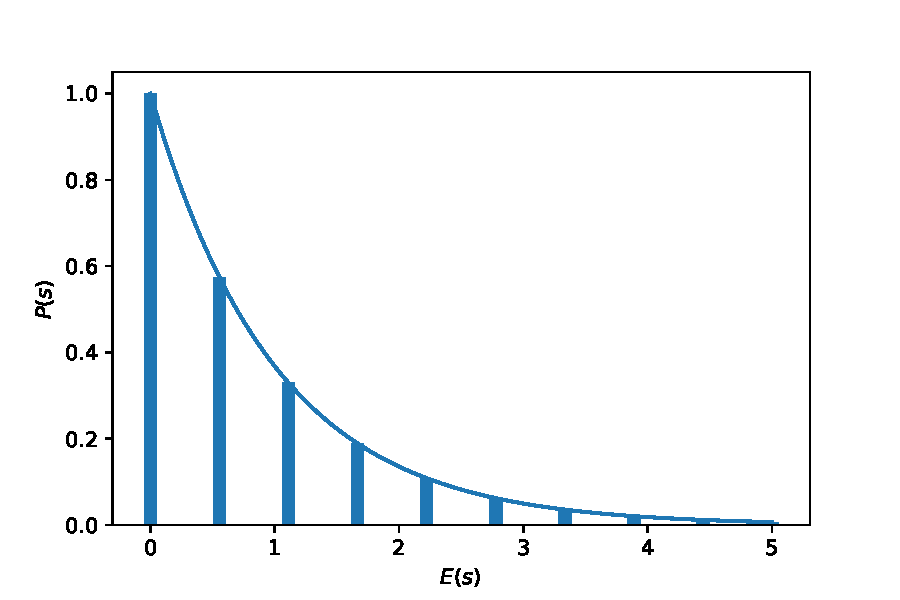
\includegraphics[width=10cm]{imgs/Boltzmann}
\caption{The probability according to the Boltzmann distribution. (1) it decays exponentially; (2) high $T$ slows down the decay. }
\end{figure}



\section{Partition Function}
Now, you are probably wondering how to calculate $Z$. The trick is to use the condition of $P(s)$,
\begin{equation}
\sum_s P(s) = \sum_s \frac{1}{Z} e^{-E(s)/kT} = \frac{1}{Z} \sum_s e^{-E(s)/kT} = 1
\end{equation}

Hence, 
\begin{equation}
Z = \sum_s e^{-E(s)/kT}
\end{equation}

The sum is not easy to carry out numerically for most of the cases. But we can take advantage of the exponential behavior to do it numerically.
When $E(s)$ goes to larger than a few $kT$, the Boltzmann factor decays very fast, thus we can simply sum a few $kT$.

The quantity $Z$ is called the {\bf partition function}. $Z$ does not depend on any particular state $s$, but it does depend on temperature. At very 
low $T$, $Z$ is approximated to 1, since all the excited states have very small Boltzmann factors. But at high temperature, $Z$ will be much larger.

{\bf Problem 6.3} Consider a hypothetical atom that has just two states, a ground state of $E$=0, and an excited state of $E$=2 eV. Draw a graph of
 the partition function for this system as a function of temperature, and evaluate the partition function numerically at $T$=[300, 3000, 30000].

\begin{figure}[h]
\centering
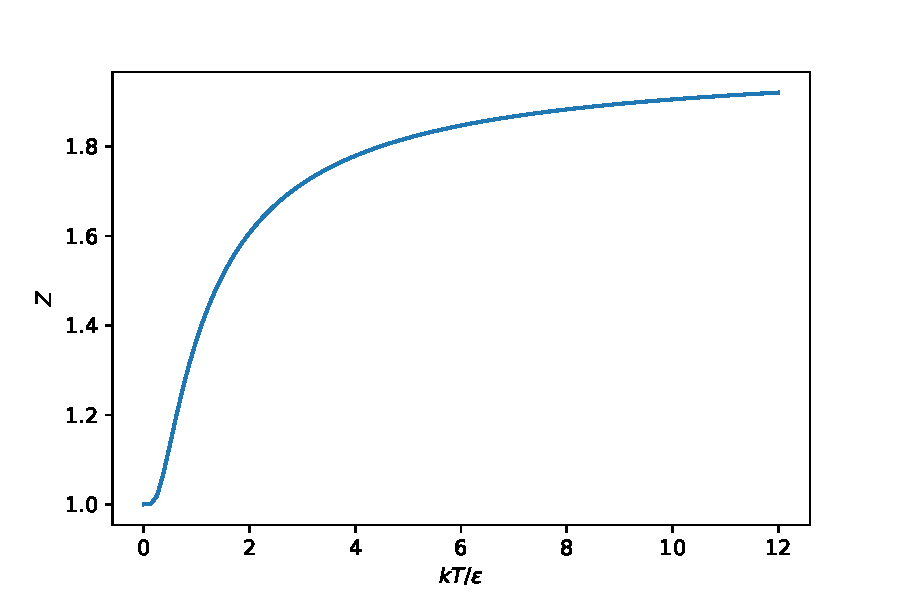
\includegraphics[width=10cm]{imgs/Partition-2s}
\caption{The partition function with respect to temperature. }
\end{figure}

